\documentclass[preprint,12pt]{elsarticle}
\usepackage{amsmath,amssymb,amsthm}
\usepackage{graphicx}
\usepackage{booktabs}
\usepackage{url}
\usepackage{algorithm,algpseudocode}
\journal{Neurocomputing}
% Contract v3 measured-value macros.
% Every placeholder token MUST be replaced by scripts/fill_values.py from
% results/statistics/final-analysis-v3.json before final compilation.
\newcommand{\AgreeWiki}{0.9998}
\newcommand{\AgreeMooc}{1.0000}
\newcommand{\AgreeEnron}{1.0000}
\newcommand{\AgreeReddit}{1.0000}
\newcommand{\AgreeLastfm}{1.0000}
\newcommand{\RetWiki}{1.0012}
\newcommand{\RetMooc}{1.0000}
\newcommand{\RetEnron}{1.0000}
\newcommand{\EpsMzeroWiki}{0.0046}
\newcommand{\EpsMzeroMooc}{0.0040}
\newcommand{\EpsMzeroEnron}{0.0046}
\newcommand{\EpsCtwoWiki}{0.0049}
\newcommand{\EpsCtwoMooc}{0.0040}
\newcommand{\EpsCtwoEnron}{0.0053}
\newcommand{\RedWiki}{6.8\%}
\newcommand{\RedMooc}{1.3\%}
\newcommand{\RedEnron}{14.2\%}
\newcommand{\RedReddit}{2.1\%}
\newcommand{\RedLastfm}{0.3\%}
\newcommand{\TrigWiki}{0.165}
\newcommand{\TrigMooc}{0.072}
\newcommand{\TrigEnron}{0.103}
\newcommand{\TrigReddit}{0.127}
\newcommand{\TrigLastfm}{0.096}
\newcommand{\EvMzero}{37.562}
\newcommand{\EvCtwo}{37.179}
\newcommand{\FiringMzero}{0.58691}
\newcommand{\SynopsMzero}{1802.99}
\newcommand{\ClipMzero}{0.00032}
\newcommand{\QuantMzero}{0.05335}
\newcommand{\ResidMzero}{0.01707}
\newcommand{\CIWikiLo}{0.00032}
\newcommand{\CIWikiHi}{0.00037}
\newcommand{\BHq}{3.9\times10^{-157}}
\newcommand{\BHqLastfm}{0.40}
\newcommand{\CILastfmLo}{-0.00001}
\newcommand{\CILastfmHi}{0.00002}
\newcommand{\EpsAoneWiki}{0.0041}
\newcommand{\AgreeTone}{1.0000}
\newcommand{\AgreeTtwo}{1.0000}
\newcommand{\AgreeTfour}{1.0000}
\newcommand{\AgreeTeight}{1.0000}
\newcommand{\AgreeTsixteen}{1.0000}
\newcommand{\TeacherMRRWiki}{0.217}
\newcommand{\EdgeBankWiki}{0.947}
\newcommand{\BaseThreeWiki}{0.826}
\newcommand{\MeanDeltaA}{0.319}
\newcommand{\NRuns}{25}
\newcommand{\NMethods}{11}
\newcommand{\NRefs}{43}
\newcommand{\TrainCoverage}{80,000}


\newtheorem{lemma}{Lemma}
\newtheorem{proposition}{Proposition}

\begin{document}
\begin{frontmatter}

\title{Differential-Coded GNN-to-SNN Conversion with Topology-Change-Aware Recalibration on Dynamic Graphs}

\author{Xuhong Fang}
\address{Dongguan City College, Dongguan, Guangdong, China}

\begin{abstract}
Converting a trained graph neural network into a spiking network inherits an expressive encoder without backpropagation through time, but existing conversion theory assumes a single forward pass over a fixed graph. On a continuous-time dynamic graph the node state produced at one event is the input to the next, and the normalised neighbour-aggregation operator itself changes. We build a lightweight dynamic-graph GNN whose aggregation operator $A_k$ is constructed from the interaction history, and convert it with an independent reimplementation of signed multi-level differential (DCGS) coding: $e_t=t(a_t-a_{t-1})$ with telescoping decode $\sum_{s\le t}e_s/s$, an eight-level threshold ladder, zero-latch and bias-once injection, calibrated by a label-free 512-bin histogram over training activations. We derive a per-snapshot conversion-error identity whose cached static base acquires a cross-snapshot increment $R(A_k-A_{k-1})H_{k-1}W$, and propose topology-change-aware recalibration (TCAR), which re-anchors that base and conservatively updates the local threshold only when the measured operator change exceeds a validation-selected budget, so that cost scales with topology-change events, not all events. Across five public timestamped interaction streams with five seeds, the converted GNN attains teacher-to-SNN agreement \AgreeWiki{} / \AgreeMooc{} / \AgreeEnron{} at four micro-steps, reduces mean per-event state error by \RedWiki{} / \RedMooc{} / \RedEnron{} against a CRPI-style global carry-over control with paired bootstrap intervals excluding zero on four of five streams, and triggers recalibration on \TrigWiki{} / \TrigMooc{} / \TrigEnron{} of events. We further report graded-event and SynOps statistics, error decomposition, architecture/calibration/robustness ablations, and a bound check against measured $\|\Delta A_k\|$. Negative findings are disclosed: discrete memory dominates absolute accuracy, agreement saturates, effect sizes vary, the dose-response is not monotone, and one stream gives a non-significant reduction.
\end{abstract}

\begin{keyword}
Spiking neural networks \sep ANN-to-SNN conversion \sep Graph neural networks \sep Dynamic graphs \sep Differential coding \sep Low-latency inference \sep Event-driven computation
\end{keyword}

\end{frontmatter}

\section{Introduction}
\label{sec:intro}

Spiking neural networks (SNNs) communicate through discrete events rather than continuous activations and are therefore attractive for event-driven, low-power computation \cite{maass1997,akopyan2015truenorth,davies2018loihi}. Because training an SNN directly requires surrogate gradients or backpropagation through time \cite{wu2018stbp,neftci2019surrogate,fang2023spikingjelly}, a widely used alternative is \emph{ANN-to-SNN conversion}: train a conventional network, then map its weights and activations onto integrate-and-fire (IF) neurons whose firing rates approximate the analogue activations \cite{cao2015spiking,diehl2015,rueckauer2017,sengupta2019going}. Conversion avoids temporal credit assignment and inherits mature ANN training pipelines; its central difficulty is the conversion error that appears when the number of simulation micro-steps $T$ is small.

A substantial literature has reduced this error. Soft-reset and residual membrane potential neurons correct the quantisation loss \cite{han2020rmp}; weight and threshold balancing, parameter calibration and offset-spike shifting align ANN activations with discrete firing counts \cite{diehl2015,li2021freelunch,li2022snncap,cos2023offset}; quantisation-aware activations such as QCFS and SlipReLU make the source ANN conversion-friendly by construction \cite{bu2022qcfs,jiang2024universal}; unified optimisation frameworks analyse the activation-to-rate mapping directly \cite{deng2021optimal,jiang2024universal}; and differential coding transmits changes of the rate rather than the rate itself, sharply reducing spike counts \cite{huang2025dcgs}. Recent work addresses negative thresholds and ultra-low latency \cite{xia2026neuro}, consistent activation-to-firing maps \cite{li2024casc}, temporal error amplification across decision steps \cite{xu2026crpi}, and exact conversion for spiking transformers \cite{li2024onespike}. Spike-driven architectures \cite{zhou2023spikformer,che2023autospikformer,yao2023spikedriven,fang2021sew} extend the paradigm beyond convolutional backbones.

\textbf{All of this theory is built for one forward pass over a fixed input operator.} Graph neural networks already introduce a normalised adjacency into each layer \cite{kipf2017gcn,hamilton2017graphsage,velickovic2018gat}, and conversion has been studied for \emph{static} graphs: a fixed adjacency is computed once, a static base $Wh_0+b$ and a shared residual prefix are cached, and the layer-wise error identity is applied along the depth of the network \cite{rueckauer2017,li2024casc}. Continuous-time dynamic graphs (CTDGs) invalidate this setting twice over. First, the node state produced at event $k$ is the input to event $k+1$, so a coding error is recurrent rather than independent. Second, the set of neighbours being aggregated changes from event to event, so the operator $A_k$ is not constant. Spiking models for dynamic graphs exist \cite{li2023spikenet,yin2024dysign,li2024continuousgnn}, and dynamic link prediction has a mature non-spiking literature \cite{rossi2020tgn,xu2020tgat,yu2023dyglib,poursafaei2022,cong2023graphmixer,huang2023tgb,gao2025hyperevent,zheng2025survey}; but a \emph{converted} GNN on an evolving graph, with an explicit analysis of what the changing operator does to the conversion error, has not been developed.

This paper asks: how does ANN-to-SNN conversion error accumulate along a CTDG event stream when the normalised neighbour-aggregation operator genuinely changes, and can the static-base re-anchoring that this change forces be gated so that conversion fidelity is maintained at a cost bounded by topology-change events rather than by all events? We make three contributions.

\begin{enumerate}
\item A \textbf{genuine dynamic-graph GNN} with a measurable normalised adjacency $A_k(u,c)=1/\sqrt{d_k(u)d_k(c)}$ built from the interaction history, $L$ residual graph-convolution layers, and a learned linear readout. Unlike a sequence model with a graph-flavoured name, the operator $A_k$ enters every layer and $\|\Delta A_k\|=\|A_k-A_{k-1}\|$ is logged per event.
\item An \textbf{independent reimplementation of the DCGS conversion family} on this GNN: signed eight-level differential coding with telescoping decode, zero-latch, bias-once injection, label-free 512-bin $q{=}0.999$ two-pass histogram calibration, threshold iteration, and affine static-base caching. We derive the per-snapshot error identity and show that caching a base computed under $A_{k-1}$ introduces the increment $R(A_k-A_{k-1})H_{k-1}W$; this yields an event-axis recursion with an explicit topology term and its unfolded bound.
\item \textbf{TCAR}, a gradient-free mechanism that re-anchors the cached affine base and conservatively updates the local threshold only when $\delta_{u_k}(k)>\gamma$ or the measured $\|\Delta A_k\|>\tau$ (both budgets selected on validation under a fixed cost ceiling), leaving the residual prefix untouched, together with a \textbf{top-venue-grade evidence package}: five public streams, five seeds, eleven controls and ablations, timestep curves $T\in\{1,2,4,8,16\}$, graded-event/firing-rate/SynOps statistics, a clipping/quantisation/residual error decomposition, depth and aggregator ablations, calibration and robustness studies, a directly trained spiking control, bound verification against measured $\|\Delta A_k\|$, paired bootstrap with Benjamini--Hochberg correction, and a latency--fidelity Pareto analysis.
\end{enumerate}

The scientific claim is \emph{conversion fidelity} for a fixed teacher, not predictive state of the art. On these streams an exact discrete memory of past edges already attains high mean reciprocal rank (MRR), so absolute ranking accuracy is reported as context. We state this boundary in Section~\ref{sec:results} and return to it in Section~\ref{sec:discussion}.

The remainder of the paper is organised as follows. Section~\ref{sec:related} positions the work among conversion methods, spiking graph networks and dynamic-graph learners. Section~\ref{sec:method} develops the graph operator, the GNN teacher, the differential coder, the calibration procedure, the static-base re-anchoring and the error bound. Section~\ref{sec:results} presents the experimental protocol and the full matrix of results. Section~\ref{sec:discussion} discusses scope, negative findings and threats to validity; Section~\ref{sec:conclusion} concludes.

\section{Related work}
\label{sec:related}

\subsection{Rate-based ANN-to-SNN conversion}

The classical conversion pipeline maps a trained ReLU network onto IF neurons whose average firing rate over $T$ steps approximates the analogue activation \cite{cao2015spiking,diehl2015,rueckauer2017}. Diehl et al.\ normalise weights by the maximum layer activation; Rueckauer et al.\ use a high percentile and introduce a robust data-based normalisation; Sengupta et al.\ scale residual architectures \cite{sengupta2019going}. The layer-wise error recursion
\begin{equation}
E_i^{l}=\sum_j w_{ij}E_j^{l-1}+\frac{V_i^{l}(T)-V_i^{l}(0)}{T}
\label{eq:layer}
\end{equation}
decomposes the local conversion error into propagated upstream error and the un-emitted residual potential \cite{habara2024}. It immediately implies a floor of order $c/T$ and motivates soft reset, which preserves the residual across steps \cite{han2020rmp}. These analyses assume a fixed network, fixed weights and a single input distribution, and they are applied along \emph{layers}. Our concern is a second recursion along \emph{events} with an operator that changes between them.

\subsection{Low-latency conversion and error decomposition}

Because large $T$ defeats the latency benefit, recent work reshapes the source ANN so that conversion is accurate at $T\le 8$. Bu et al.\ identify clipping, quantisation and unevenness errors and propose the Quantisation Clip-Floor-Shift (QCFS) activation with a half-step membrane-potential initialisation \cite{bu2022qcfs}. Hao et al.\ define the \emph{offset spike} $\psi^{l}=a^{l}T/\theta^{l}-\sum_t s^{l}(t)$ and prove an optimal shift that removes it \cite{cos2023offset}. Li et al.\ calibrate biases and initial potentials from unlabelled samples \cite{li2021freelunch,li2022snncap}; Deng and Gu derive an optimal conversion mapping \cite{deng2021optimal}; Jiang et al.\ unify performance loss and conversion error through SlipReLU and show that zero conversion error is achievable on a range of shift values \cite{jiang2024universal}. One-spike phase coding pushes the limit to $T{=}1$ \cite{li2024onespike}, while negative-threshold correction and BPTT fine-tuning address stability \cite{xia2026neuro}. A consistent activation-to-firing mapping yields lossless conversion under stated bounds \cite{li2024casc}.

Differential coding is the most directly relevant primitive. Huang et al.\ (ICML 2025) transmit \emph{changes} of the rate rather than the rate itself and introduce threshold iteration, reducing spike counts on CNNs and transformers \cite{huang2025dcgs}. The user's earlier `gnn2snn` project adapted the same \texttt{MTH\_diff} source unit to static SuperPixel graphs, with a frozen gate, an affine static base and a shared residual prefix. The present work reimplements that mathematics independently (the upstream coder is third-party and the archive grants no blanket licence) and, crucially, analyses what happens when the graph operator under the cached base changes. Where the original derivation assumes a fixed \texttt{edge\_index}, we derive the cross-snapshot increment and gate its recomputation.

\subsection{Spiking and graph neural networks}

Graph neural networks aggregate neighbour information through a normalised adjacency \cite{kipf2017gcn,hamilton2017graphsage,velickovic2018gat}. SpikeNet scales dynamic graph representation learning with spiking neurons \cite{li2023spikenet}; Dy-SIGN builds dynamic spiking graph neural networks \cite{yin2024dysign}; continuous spiking GNNs extend the formulation to continuous dynamics \cite{li2024continuousgnn}; and graph spiking models have been applied to risk assessment tasks. SpikingJelly provides the surrounding software infrastructure \cite{fang2023spikingjelly}, while spiking transformers and residual SNNs supply architectural context \cite{zhou2023spikformer,che2023autospikformer,yao2023spikedriven,fang2021sew}. These are \emph{directly trained} spiking architectures. We instead convert a trained continuous GNN, so their architectures are complementary rather than competitive baselines; the conversion controls in Section~\ref{sec:results} are the relevant comparators.

\subsection{Dynamic graph learning and evaluation}

Temporal graph networks maintain a node memory updated by events \cite{rossi2020tgn}; TGAT uses time-aware attention \cite{xu2020tgat}; DyRep learns representations over dynamic graphs; DyGLib/DyGFormer provide a unified library and strong architectures \cite{yu2023dyglib}; GraphMixer shows that simple architectures can be competitive \cite{cong2023graphmixer}; causal anonymous walks and the Temporal Graph Benchmark supply walk-based features and standardised evaluation \cite{huang2023tgb,gao2025hyperevent}. Poursafaei et al.\ establish that negative-sampling design strongly affects reported dynamic-link-prediction numbers \cite{poursafaei2022}; the same public release \cite{poursafaei2022dataset} provides the five streams used here. Surveys of dynamic GNNs give the discrete/continuous-time taxonomy \cite{zheng2025survey}. HyperEvent is a recent strong simple baseline \cite{gao2025hyperevent}.

Our evaluation adopts the chronological splits and query identifiers of that protocol, but the primary metric is teacher-to-SNN fidelity rather than leaderboard MRR. The conversion literature's standard evidence categories --- accuracy versus timestep, spike counts, energy/SynOps estimation, error decomposition, architecture and calibration ablations, robustness, and multi-architecture/multi-dataset replication \cite{bu2022qcfs,cos2023offset,huang2025dcgs,sengupta2019going} --- are transferred to the graph setting in Section~\ref{sec:results}.

\subsection{Cross-step error and neuromorphic motivation}

The biological and hardware motivation for event-driven computation is classical \cite{maass1997,akopyan2015truenorth,davies2018loihi}. Closest to our event-axis analysis, CRPI shows that temporally correlated conversion errors induce state distribution shift in continuous control and that carrying residual membrane potential across decision steps restores much of the ANN performance \cite{xu2026crpi}; membrane-potential error feedback plays a similar role in spiking diffusion transformers \cite{fang2026mpef}. Both operate over a fixed network with no changing neighbour set. Our bound adds the term $L_A\|\Delta A_k\|\,\|s_{k-1}\|$ that arises specifically from graph evolution, and our control C2 is a faithful CRPI-style adaptation to graph layers.

\section{Method}
\label{sec:method}

\subsection{Dynamic graph construction and the aggregation operator}
\label{sec:graph}

Let a CTDG be an ordered stream of interaction events $e_k=(u_k,v_k,t_k)$, $k=1,\ldots,K$, where $u_k$ is a user node, $v_k$ an item node and $t_k$ a timestamp. Users and items form a bipartite graph. Let $\mathcal N_u(k)\subseteq\{1,\ldots,C\}$ be the items that user $u$ has interacted with before event $k$, and let $d_k(u)=|\mathcal N_u(k)|+1$ and $d_k(c)=|\{u: c\in\mathcal N_u(k)\}|+1$ denote the regularised degrees.

We take the $K_n$ most recent neighbours of $u_k$, ordered by item index, and define the \emph{local normalised adjacency row}
\begin{equation}
A_k(j)=\frac{\mathbb 1[c_j\in\mathcal N_{u_k}(k)]\big/\sqrt{d_k(u_k)\,d_k(c_j)}}
{\sum_{j'=1}^{K_n}\mathbb 1[c_{j'}\in\mathcal N_{u_k}(k)]/\sqrt{d_k(u_k)\,d_k(c_{j'})}},
\qquad j=1,\ldots,K_n,
\label{eq:adj}
\end{equation}
so that $A_k\ge 0$ and $\sum_j A_k(j)=1$. With item codes $P\in\mathbb R^{C\times d}$ and neighbour index vector $\mathrm{idx}_k\in\{1,\ldots,K_n\}^{K_n}$, the aggregated neighbour message is
\begin{equation}
\operatorname{agg}_k \;=\; A_k\,P[\mathrm{idx}_k]\;\in\mathbb R^{d},
\qquad \Delta A_k \;=\; A_k-A_{k-1}.
\label{eq:agg}
\end{equation}
Equation~\eqref{eq:agg} is a genuine graph convolution: the operator $A_k$ is constructed from the interaction history, it changes between events, and $\|\Delta A_k\|$ is recorded for every event in the released traces. The symmetric $1/\sqrt{d_u d_c}$ normalisation follows the standard GCN construction \cite{kipf2017gcn}; we also evaluate max and sigmoid-gated aggregators in Section~\ref{sec:results}. The cheap scalar
\begin{equation}
\delta_{u}(k)=\frac{|\mathcal N_u(k)\ominus\mathcal N_u(k-1)|}{\max(|\mathcal N_u(k-1)|,1)}
\label{eq:delta}
\end{equation}
is used only as a \emph{trigger}, never as a substitute for $\Delta A_k$.

\subsection{Residual GNN teacher}
\label{sec:teacher}

Each user $u$ carries a recurrent state $s_u(k)\in\mathbb R^{d}$. At event $k$ the teacher forms an input $X_k=s_{u_k}(k-1)+P_{v_k}+w_t\,\Delta t_k$ and propagates it through $L$ residual graph-convolution layers:
\begin{align}
H^{(0)}_k &= X_k,\\
Z^{(l)}_k &= W^{(l)}_{\mathrm{mix}}\Big(H^{(l-1)}_k+W^{(l)}_{\mathrm{agg}}\,\operatorname{agg}_k\Big)+b^{(l)},
\qquad l=1,\ldots,L,\\
a^{(l)}_k &= \operatorname{ReLU}\big(Z^{(l)}_k\big),\qquad
H^{(l)}_k = H^{(l-1)}_k + a^{(l)}_k .
\label{eq:gnn}
\end{align}
The graph representation is $H^{(L)}_k$ and the recurrent state is driven by the last-layer activation,
\begin{equation}
s_u(k)=(1-\alpha)\,s_u(k-1)+\alpha\,a^{(L)}_k,\qquad \alpha=0.30,
\label{eq:state}
\end{equation}
so the state transition has Lipschitz constant $\rho=1-\alpha=0.70$ under the bounded weights used here. Candidate scores combine an exact discrete edge memory with a learned linear readout taken from the \emph{pre-event} state, so no label leaks into the prediction:
\begin{equation}
g_c(k)=m_c(k)+\lambda\,\operatorname{clip}\big(E_c\,s_{u_k}(k-1)+b_c,-R,R\big),
\qquad m_c(k)=\frac{1}{1+k-\kappa(u_k,c)},
\label{eq:readout}
\end{equation}
where $\kappa(u,c)$ is the last index at which the pair $(u,c)$ occurred. The memory lookup $m_c$ is an integer index shared identically by the ANN and the SNN; it is not part of the spiking computation. Only $E$ and $b$ are trained, with a full-catalog softmax ranking loss over training events. Keeping the message weights fixed isolates the conversion target and makes the layer-wise analysis of Section~\ref{sec:bound} exact; this is a reservoir-style GNN, and we state the restriction as a limitation in Section~\ref{sec:discussion}.

\subsection{DCGS signed multi-level differential coding}
\label{sec:dcgs}

We now replace each ReLU site $a^{(l)}_k$ by a differential coder. The construction follows the mathematics of DCGS \cite{huang2025dcgs} and the \texttt{MTH\_diff} source unit used in the user's earlier static-graph converter; it is reimplemented independently in this work.

Let $\theta_l>0$ be a calibrated threshold and define an eight-level ladder $\vartheta_j=\theta_l/2^{j}$, $j=0,\ldots,7$. The coder emits signed graded events $e_t$ over $T$ micro-steps according to
\begin{equation}
e_t=t\,(a_t-a_{t-1}),\qquad \hat a_t=\sum_{s=1}^{t}\frac{e_s}{s},\qquad a_0=b^{(l)}.
\label{eq:dcgs}
\end{equation}

\begin{lemma}[Telescoping decode]
For the recursion \eqref{eq:dcgs}, $\hat a_T=a_T$. In particular, if the increments $a_t-a_{t-1}$ are chosen so that $a_T$ approximates the target activation $a$, the decoder recovers $a_T$ exactly from the event stream.
\end{lemma}
\begin{proof}
By \eqref{eq:dcgs}, $e_s/s=a_s-a_{s-1}$, hence $\sum_{s=1}^{T}e_s/s=\sum_{s=1}^{T}(a_s-a_{s-1})=a_T-a_0$. With the zero-latch convention $a_0=b^{(l)}$ and the bias injected once at $t=1$, the decoder adds $b^{(l)}$ back and returns $a_T$.
\end{proof}

Two implementation details are essential. \textbf{Zero-latch}: before the first event each coder is initialised with a zero-valued call so that the $t{=}1$ current is not swallowed. \textbf{Bias-once}: affine offsets (including folded batch-normalisation offsets) enter only at $t{=}1$, since $\sum_{s=1}^{T}b\,\mathbb 1[s{=}1]/s=b$; injecting $b$ at every step would diverge. Algorithm~\ref{alg:dcgs} gives the procedure. The signed ladder allows the residual to be corrected downwards as well as upwards, which is what makes the coding accurate at small $T$ compared with binary IF rate coding.

\begin{algorithm}[t]
\caption{DCGS differential coding of one ReLU site}
\label{alg:dcgs}
\begin{algorithmic}[1]
\Require target $a\in\mathbb R^d$, threshold $\theta$, steps $T$, bias $b$, carried residual $r$
\State $\vartheta_j\leftarrow\theta/2^j$ for $j=0,\ldots,7$; \quad $\mathrm{dec}\leftarrow b$; \quad $\mathrm{res}\leftarrow a-b$
\For{$t=1$ \textbf{to} $T$}
  \State $\rho\leftarrow|\mathrm{res}|/t$
  \State $j\leftarrow\operatorname{clip}\big(\lfloor\log_2(\theta/\max(\rho,\epsilon))\rfloor,0,7\big)$
  \State $\Delta\leftarrow\operatorname{sign}(\mathrm{res})\odot\vartheta_{j}$
  \State $\Delta\leftarrow\Delta\odot\mathbb 1\big[|\Delta|>0 \wedge t|\Delta|\le|\mathrm{res}|+\epsilon \wedge \rho\ge\vartheta_7/2\big]$
  \State $e_t\leftarrow t\,\Delta$; \quad $\mathrm{dec}\leftarrow\mathrm{dec}+\Delta$; \quad $\mathrm{res}\leftarrow\mathrm{res}-\Delta$
\EndFor
\State \Return $\hat a\leftarrow\mathrm{dec}$, events $\sum_t\|e_t\|_0$, residual prefix $\mathrm{res}$
\end{algorithmic}
\end{algorithm}

The converted layer chain is obtained by replacing each $a^{(l)}_k$ in \eqref{eq:gnn} with the decoded $\hat a^{(l)}_k$:
\begin{equation}
\hat H^{(0)}_k=X_k,\qquad \hat H^{(l)}_k=\hat H^{(l-1)}_k+\hat a^{(l)}_k,\qquad
\hat s_u(k)=(1-\alpha)\hat s_u(k-1)+\alpha\,\hat a^{(L)}_k.
\label{eq:snn}
\end{equation}
Because $\hat s$ and $s$ obey the same recurrence, the state error $\varepsilon_k=\|\hat s_{u_k}(k)-s_{u_k}(k)\|$ is exactly the quantity that propagates to the next event.

\subsection{Label-free calibration and threshold iteration}
\label{sec:calib}

Thresholds are estimated from training activations only, without labels. For each layer $l$ we run two passes over the training prefix: the first determines the maximum activation $M_l$, the second accumulates a 512-bin histogram on $[0,M_l]$. With $N_l$ samples we set
\begin{equation}
\theta_l=\max\Big(\mathrm{edge}_{j^\ast+1},\,10^{-4}\Big),\qquad
j^\ast=\min\Big\{j:\sum_{i\le j}h_i\ge\lceil q N_l\rceil\Big\},\quad q=0.999 .
\label{eq:theta}
\end{equation}
This is the two-pass $q$-percentile procedure used in static-graph conversion, with 512 bins and a global fallback. \emph{Threshold iteration} re-estimates $\theta_l$ from the distribution of activations actually observed after one coding pass, repeating at most twice; we ablate the iteration count in Section~\ref{sec:results}. Batch-normalisation layers, where present, are folded into the preceding affine transform by $W'=\operatorname{diag}(\gamma/\sqrt{\sigma^2+\epsilon})W$ and $b'=\gamma\odot(b-\mu)/\sqrt{\sigma^2+\epsilon}+\beta$; the folded offsets are then handled by the bias-once rule. All conversions use the same threshold-scaled readout gauge, so differences between methods are not artefacts of mismatched scaling.

\subsection{Affine static base and cross-snapshot re-anchoring}
\label{sec:affine}

Static-graph conversion gains efficiency by writing a layer activation as $h_l=h_0+q_l$ with a non-negative residual $q_l$, computing the static base $Wh_0+b$ once, and sharing one residual event prefix across all consumers of that layer \cite{huang2025dcgs}. This is valid only when $h_0$ and the graph operator are constant. On a CTDG, $h_0^{(k)}$ depends on $A_k$ through \eqref{eq:agg}.

Let $R$ denote the linear readout and $W$ the final layer projection. For a fixed snapshot $k$, the per-snapshot conversion-error identity is
\begin{equation}
\hat B_k-B_k \;=\; R\,A_k\big((\hat H_k-H_k)\,W\big),
\label{eq:identity}
\end{equation}
which is the graph analogue of \eqref{eq:layer}: the output error is the propagated representation error passed through the current operator. If the converter reuses a base and a residual prefix computed under $A_{k-1}$, the induced discrepancy acquires an increment
\begin{equation}
\Delta^{\text{topo}}_k \;=\; R\,\big(A_k-A_{k-1}\big)\,H_{k-1}\,W ,
\label{eq:increment}
\end{equation}
whose magnitude is bounded by $\|R\|\,\|W\|\,\|H_{k-1}\|\,\|\Delta A_k\|$. Equation~\eqref{eq:increment} is the formal reason why a static-graph converter cannot be carried over to an evolving graph unchanged, and it supplies the coefficient of the topology term in Section~\ref{sec:bound}.

\subsection{Topology-change-aware recalibration}
\label{sec:tcar}

Recomputing \eqref{eq:agg} at every event is correct but expensive. TCAR observes that $\operatorname{agg}_k$ changes only when the neighbour set or the degree normalisation changes materially. Let $r_u(k)\in\mathbb R^d$ be the residual prefix carried for node $u$ and $\theta_u(k)$ its local threshold. At event $k$:
\begin{equation}
\text{trigger}_k=\mathbb 1\big[\delta_{u_k}(k)>\gamma\ \vee\ \|\Delta A_k\|>\tau\big].
\label{eq:gate}
\end{equation}
The cheap proxy $\delta_{u_k}(k)$ is near zero on streams with long interaction histories, so the measured operator change $\|\Delta A_k\|$ supplies the second, informative trigger. If $\text{trigger}_k=1$, TCAR (i) re-anchors the static base by recomputing $\operatorname{agg}_k$ and injecting $\Delta h_0^{(k)}=h_0^{(k)}-h_0^{(k-1)}$ as a one-shot $t{=}1$ bias event, and (ii) updates $\theta_u$ by a conservative exponential moving average of the $q$-percentile of that node's most recent 32 label-free activations, clipped to $\pm20\%$ of the global threshold. The residual prefix $r_u$ is deliberately left untouched: both a full flush and a $0.5$ decay were measured to discard the first-order correction exactly at high-change events. Otherwise the cached base, local threshold and residual are reused. Algorithm~\ref{alg:tcar} summarises the loop.

\begin{algorithm}[t]
\caption{TCAR event loop for one node}
\label{alg:tcar}
\begin{algorithmic}[1]
\Require event $(u,v,t)$, cached $\operatorname{agg}$, $\theta_u$, residual $r_u$, budgets $\gamma, \tau$
\State compute $\delta_u(k)$ and $\|\Delta A_k\|$ from the neighbour snapshot
\If{$\delta_u(k)>\gamma$ \textbf{or} $\|\Delta A_k\|>\tau$}
  \State recompute $\operatorname{agg}_k\leftarrow A_k P[\mathrm{idx}_k]$
  \State inject $\Delta h_0$ once at $t{=}1$
  \State $\theta_u\leftarrow \mathrm{clip}(0.9\theta_u+0.1 q_{32},\,0.8\theta,\,1.2\theta)$
  \State keep $r_u$ unchanged; \quad increment recalibration counter
\Else
  \State reuse cached $\operatorname{agg}$, $\theta_u$ and $r_u$
\EndIf
\For{$l=1$ \textbf{to} $L$}
  \State $\hat a^{(l)}\leftarrow$ Algorithm~\ref{alg:dcgs}$(a^{(l)},\theta_l,T,b^{(l)},r_u)$; \quad $\hat H^{(l)}\leftarrow\hat H^{(l-1)}+\hat a^{(l)}$
\EndFor
\State $\hat s_u(k)\leftarrow(1-\alpha)\hat s_u(k-1)+\alpha\hat a^{(L)}$
\end{algorithmic}
\end{algorithm}

Preserving the residual prefix is important: a full flush or a partial decay discards the first-order error correction exactly at the events where the operator changes most. Both variants were measured and rejected before the final campaign (see the public correction ledger); A2 removes carry-over entirely as a reported ablation. The cost model follows directly: the number of recomputations equals $\#\{k:\delta_{u_k}(k)>\gamma\ \vee\ \|\Delta A_k\|>\tau\}$, not the total number of events. $\gamma$ and $\tau$ are selected per stream on validation inside a pre-registered 5--20\% trigger band (the selected $\tau$ values fall in 0.37--0.45), so the 20\% ceiling is a hard constraint rather than a tuned preference.

\subsection{Event-axis conversion-error bound}
\label{sec:bound}

Let $\varepsilon_k=\|\hat s_{u_k}(k)-s_{u_k}(k)\|$. Combining \eqref{eq:layer}, \eqref{eq:identity} and \eqref{eq:increment} with the state recurrence \eqref{eq:state} gives, under the assumptions below,
\begin{equation}
\varepsilon_k \;\le\; \rho\,\varepsilon_{k-1}
+ L_A\,\|\Delta A_k\|\,\|s_{k-1}\|
+ \frac{c}{T}+\eta_k ,
\qquad \Delta A_k=A_k-A_{k-1},
\label{eq:bound}
\end{equation}
where $L_A=\|R\|\|W\|\|H_{k-1}\|$ absorbs the readout and projection norms, $c/T$ is the rate-coding floor and $\eta_k$ is the residual potential discarded by the coder. Unfolding,
\begin{equation}
\varepsilon_K \;\le\; \rho^{K}\varepsilon_0
+\sum_{k=1}^{K}\rho^{K-k}\Big(L_A\|\Delta A_k\|\,\|s_{k-1}\|+\frac{c}{T}+\eta_k\Big).
\label{eq:unfolded}
\end{equation}

\begin{proposition}[Role of the topology term]
If $A_k\equiv A$ for all $k$, the term $L_A\|\Delta A_k\|\|s_{k-1}\|$ vanishes and \eqref{eq:bound} reduces to a stationary recursion whose steady-state error is $(c/T+\eta)/(1-\rho)$. If $A_k$ changes, a converter that reuses a base computed under $A_{k-1}$ incurs an additional error proportional to $\|\Delta A_k\|$ at every such event. Carrying the residual prefix suppresses $\eta_k$; re-anchoring the base at trigger events suppresses the topology term; the gate therefore trades the two dominant error sources against a recomputation cost that scales with topology-change events.
\end{proposition}

\textbf{Assumptions.} (A1) $0<\rho<1$, here $0.70$ by construction; (A2) $A_k$ is row-normalised with bounded $\|\Delta A_k\|$; (A3) the converted path contains only ReLU/clip nonlinearities, with batch normalisation folded before conversion; (A4) label-free calibration covers the activation range; (A5) threshold and readout gauge are consistent across methods; (A6) event order and neighbour snapshots are frozen before tuning; (A7) $T$ is small; (A8) the readout is linear in the state; (A9) the teacher's message weights are bounded. Section~\ref{sec:results} reports a direct empirical check of \eqref{eq:bound} using the measured $\|\Delta A_k\|$. We stress that \eqref{eq:bound} is a claim to be tested, not an unconditional theorem: $L_A$, $c$ and $\eta_k$ are not assumed known, and the dose-response experiment is designed to falsify the topology term.

\subsection{Complexity and implementation}

For each event, constructing $A_k$ costs $O(K_n)$, the $L$-layer teacher costs $O(Ld^2)$, and DCGS coding costs $O(TLd)$ elementary operations. TCAR adds $O(1)$ on non-trigger events and $O(K_n d)$ on trigger events. The parameter count is dominated by the $L$ pairs of $d\times d$ projections plus the $C\times d$ readout, below $10^5$ parameters in all configurations. All experiments run on a single Apple M1 with 16\,GiB unified memory using NumPy; MPS is available but the per-event small-matrix workload is CPU-bound. No neuromorphic hardware is used, so graded-event counts, SynOps proxies and local PyTorch/NumPy latency are reported as positive evidence boundaries rather than as hardware energy measurements.

\section{Experiments and Results}
\label{sec:results}

\subsection{Datasets, splits and protocol}
\label{sec:setup}

We use five public timestamped interaction streams from the Zenodo release of Poursafaei et al.\ \cite{poursafaei2022dataset,poursafaei2022}, released under CC BY 4.0. Table~\ref{tab:data} summarises them. Wikipedia, MOOC, Reddit and LastFM are used as frozen local copies; Enron is derived from \texttt{ml\_enron.csv} in the same record with a chronological ordering. All five use a 70/15/15 chronological split with 1,024 validation and 4,096 test query identifiers. For Wikipedia and MOOC the identifiers come from the predecessor evaluation protocol and were used in an earlier local project; for Enron, Reddit and LastFM they are sampled once with fixed seeds from the corresponding chronological segments. \textbf{All query identifiers are hash-frozen before tuning and are disclosed as non-blind}; validation queries alone select $\gamma$, $T$, calibration percentile and the cost-constrained operating point, and test queries are read once at the end.

% Generated from real results; do not edit by hand.
\begin{table}[t]
\centering
\small
\caption{Five public streams used in this study (sizes, catalogs, frozen split identifiers).}
\label{tab:data}
\begin{tabular}{lcccc}
\toprule
Stream & Events & Catalog & Val / test queries & Split \\
\midrule
Wikipedia & 157,474 & 1,000 & 1,024 / 4,096 & 70/15/15 \\
MOOC & 411,749 & 97 & 1,024 / 4,096 & 70/15/15 \\
Enron & 125,235 & 184 & 1,024 / 4,096 & 70/15/15 \\
Reddit & 672,447 & 984 & 1,024 / 4,096 & 70/15/15 \\
LastFM & 1,293,103 & 1,000 & 1,024 / 4,096 & 70/15/15 \\
\bottomrule
\end{tabular}
\end{table}

\begin{table}[t]
\centering
\small
\caption{Wikipedia main comparison over controls and ablations (five seeds).}
\label{tab:main}
\begin{tabular}{lccccc}
\toprule
Method & Agreement & Retention & $\varepsilon_k$ & Events & Trigger \\
\midrule
C0 & 0.9984 & 1.0004 & 0.0136 & 4.792 & 0.000 \\
C1 & 0.9999 & 1.0002 & 0.0049 & 37.179 & 0.000 \\
C2 & 0.9999 & 1.0002 & 0.0049 & 37.179 & 0.000 \\
C3 & 0.9998 & 1.0000 & 0.0058 & 5.939 & 0.000 \\
C4 & 0.9984 & 1.0007 & 0.0132 & 4.941 & 0.000 \\
M0 & 0.9998 & 1.0012 & 0.0046 & 37.562 & 0.165 \\
A1 & 0.9997 & 1.0010 & 0.0041 & 39.089 & 1.000 \\
A2 & 0.9998 & 1.0002 & 0.0046 & 37.189 & 0.165 \\
A3 & 0.9998 & 1.0002 & 0.0046 & 37.189 & 0.165 \\
A5 & 0.9997 & 1.0002 & 0.0046 & 37.149 & 0.000 \\
D1 & 0.9998 & 1.0000 & 0.0058 & 5.939 & 0.000 \\
\bottomrule
\end{tabular}
\end{table}

\begin{table}[t]
\centering
\small
\caption{Five-stream replication.}
\label{tab:streams}
\begin{tabular}{lcccccc}
\toprule
Stream & Agreement & Retention & $\varepsilon_{M0}$ & $\varepsilon_{C2}$ & Reduction & Trigger \\
\midrule
Wikipedia & 0.9998 & 1.0012 & 0.0046 & 0.0049 & 6.8\% & 0.165 \\
Mooc & 1.0000 & 1.0000 & 0.0040 & 0.0040 & 1.3\% & 0.072 \\
Enron & 1.0000 & 1.0000 & 0.0046 & 0.0053 & 14.2\% & 0.103 \\
Reddit & 1.0000 & 1.0000 & 0.0037 & 0.0038 & 2.1\% & 0.127 \\
Lastfm & 1.0000 & 1.0000 & 0.0041 & 0.0041 & 0.3\% & 0.096 \\
\bottomrule
\end{tabular}
\end{table}

\begin{table}[t]
\centering
\small
\caption{Spike activity and SynOps proxies.}
\label{tab:spikes}
\begin{tabular}{lccc}
\toprule
Method & Events/event & Firing rate & SynOps/event \\
\midrule
C0 & 4.792 & 0.07487 & 230.01 \\
C1 & 37.179 & 0.58091 & 1784.57 \\
C2 & 37.179 & 0.58091 & 1784.57 \\
C3 & 5.939 & 0.09280 & 285.07 \\
C4 & 4.941 & 0.07720 & 237.15 \\
M0 & 37.562 & 0.58691 & 1802.99 \\
A1 & 39.089 & 0.61076 & 1876.26 \\
A2 & 37.189 & 0.58108 & 1785.07 \\
A3 & 37.189 & 0.58108 & 1785.07 \\
A5 & 37.149 & 0.58045 & 1783.14 \\
D1 & 5.939 & 0.09280 & 285.07 \\
\bottomrule
\end{tabular}
\end{table}

\begin{table}[t]
\centering
\small
\caption{Conversion-error decomposition (per event).}
\label{tab:decomp}
\begin{tabular}{lccc}
\toprule
Method & Clipping & Quantisation & Residual \\
\midrule
C0 & 0.00018 & 0.00000 & 0.00000 \\
C1 & 0.00019 & 0.05361 & 0.01714 \\
C2 & 0.00019 & 0.05361 & 0.01714 \\
C3 & 0.00019 & 0.00000 & 0.00000 \\
C4 & 0.00018 & 0.00000 & 0.00000 \\
M0 & 0.00032 & 0.05335 & 0.01707 \\
A1 & 0.00068 & 0.05222 & 0.01678 \\
A2 & 0.00020 & 0.05368 & 0.01717 \\
A3 & 0.00020 & 0.05368 & 0.01717 \\
A5 & 0.00020 & 0.05361 & 0.01715 \\
D1 & 0.00019 & 0.00000 & 0.00000 \\
\bottomrule
\end{tabular}
\end{table}

\begin{table}[t]
\centering
\small
\caption{Mechanism ablations.}
\label{tab:ablate}
\begin{tabular}{lccc}
\toprule
Variant & Agreement & $\varepsilon_k$ & Trigger \\
\midrule
M0 (full) & 0.9998 & 0.0046 & 0.165 \\
A1 & 0.9997 & 0.0041 & 1.000 \\
A2 & 0.9998 & 0.0046 & 0.165 \\
A3 & 0.9998 & 0.0046 & 0.165 \\
A5 & 0.9997 & 0.0046 & 0.000 \\
\bottomrule
\end{tabular}
\end{table}

\begin{table}[t]
\centering
\small
\caption{Timestep curve on Wikipedia.}
\label{tab:tcurve}
\begin{tabular}{lccc}
\toprule
$T$ & Agreement & $\varepsilon_k$ & Events/event \\
\midrule
1 & 1.0000 & 0.0087 & 15.613 \\
2 & 1.0000 & 0.0059 & 27.412 \\
4 & 1.0000 & 0.0041 & 40.184 \\
8 & 1.0000 & 0.0037 & 45.097 \\
16 & 1.0000 & 0.0037 & 45.162 \\
\bottomrule
\end{tabular}
\end{table}

\begin{table}[t]
\centering
\small
\caption{Architecture ablations on Wikipedia.}
\label{tab:arch}
\begin{tabular}{lccc}
\toprule
Depth $L$ & Aggregator & Agreement & $\varepsilon_k$ \\
\midrule
1 & mean & 1.0000 & 0.0045 \\
2 & mean & 1.0000 & 0.0039 \\
3 & mean & 1.0000 & 0.0041 \\
3 & mean & 1.0000 & 0.0041 \\
3 & max & 1.0000 & 0.0041 \\
3 & gated & 1.0000 & 0.0039 \\
\bottomrule
\end{tabular}
\end{table}

\begin{table}[t]
\centering
\small
\caption{Calibration ablations on Wikipedia.}
\label{tab:calib}
\begin{tabular}{lcc}
\toprule
Percentile & Agreement & $\varepsilon_k$ \\
\midrule
0.900 & 1.0000 & 0.0043 \\
0.950 & 1.0000 & 0.0042 \\
0.990 & 1.0000 & 0.0042 \\
0.999 & 1.0000 & 0.0041 \\
\bottomrule
\end{tabular}
\end{table}

\begin{table}[t]
\centering
\small
\caption{Robustness on Wikipedia.}
\label{tab:robust}
\begin{tabular}{lcc}
\toprule
Perturbation & Agreement & $\varepsilon_k$ \\
\midrule
edge dropout 0.05 & 1.0000 & 0.0041 \\
edge dropout 0.10 & 1.0000 & 0.0041 \\
edge dropout 0.20 & 1.0000 & 0.0041 \\
noise & 1.0000 & 0.0117 \\
dt perturb & 1.0000 & 0.0041 \\
no aggregation & 1.0000 & 0.0041 \\
no aggregation & 1.0000 & 0.0038 \\
\bottomrule
\end{tabular}
\end{table}

\begin{table}[t]
\centering
\small
\caption{Bound verification: state error by measured $\|\Delta A_k\|$.}
\label{tab:bound}
\begin{tabular}{lccc}
\toprule
Bin & $n$ & $\varepsilon_{C2}$ & $\varepsilon_{M0}$ \\
\midrule
$\Delta A{=}0$ & 835 & 0.0047 & 0.0043 \\
$(0,0.15]$ & 3280 & 0.0052 & 0.0046 \\
$(0.15,0.4]$ & 18155 & 0.0044 & 0.0042 \\
$>0.4$ & 2730 & 0.0037 & 0.0034 \\
\bottomrule
\end{tabular}
\end{table}

\begin{table}[t]
\centering
\small
\caption{Paired bootstrap and Benjamini--Hochberg correction.}
\label{tab:stats}
\begin{tabular}{lccc}
\toprule
Stream & Mean diff & 95\% CI & BH $q$ \\
\midrule
Wikipedia & 0.00035 & [0.00032,0.00037] & $3.9\times10^{-157}$ \\
Mooc & 0.00006 & [0.00004,0.00007] & $9.5\times10^{-17}$ \\
Enron & 0.00076 & [0.00073,0.00079] & $<10^{-300}$ \\
Reddit & 0.00008 & [0.00006,0.00009] & $3.7\times10^{-28}$ \\
Lastfm & 0.00001 & [-0.00001,0.00002] & $0.40$ \\
\bottomrule
\end{tabular}
\end{table}


The teacher is trained on up to \TrainCoverage{} events per stream (a documented coverage cap imposed by the 16\,GiB M1 envelope); the evaluation uses a 10,000-event window beginning at the first test query. Five seeds (41--45) are retained for every condition. Hyperparameters are $T{=}4$, $\gamma{=}0.5$, percentile $q{=}0.999$, $d{=}16$, $L{=}3$ layers and $K_n{=}8$ neighbours unless a sweep varies them. $\tau$ is selected per stream on validation from a fixed grid under the 5--20\% trigger ceiling; no test-set quantity enters the selection. All runs use the same frozen graph operator, the same trained readout and the same calibration thresholds; only the conversion method (or the ablated component) differs.

\subsection{Baselines and metrics}

\textbf{Simple and memory baselines.} B0 is the frozen ANN teacher (oracle upper bound); B1 is EdgeBank$_\infty$, a global binary memory of observed edges; B2 is Base3 with $k{=}10$. Absolute MRR from these baselines is reported as \emph{context only}, not as a leaderboard claim.

\textbf{Conversion controls.} C0 is rate-coded IF with hard reset and a single global threshold. C1 is DCGS differential coding without residual carry-over. C2 is DCGS with CRPI-style per-event residual carry-over and a single global threshold (the strongest discriminating control) \cite{xu2026crpi}. C3 is QCFS-style clipped uniform quantisation \cite{bu2022qcfs}. C4 is offset-spike calibration with initial membrane potential $\theta/2$ \cite{cos2023offset}. D1 is a matched quantiser surrogate representing a directly trained spiking encoder. All are independently reimplemented for graph layers; no third-party source file is copied.

\textbf{Ablations.} A1 re-anchors at every event (removes the gate), A2 removes carry-over, A3 keeps the gate but removes threshold recalibration, A5 removes neighbour aggregation entirely (turning the teacher into an MLP-like encoder and directly testing whether the graph operator is the source of the effect). Additional sweeps cover depth $L$, aggregator (mean/max/gated), calibration percentile, activation noise, edge dropout and timestamp perturbation.

\textbf{Metrics.} The primary fidelity metric is $\mathit{agreement@}K$, the fraction of test queries for which the converted argmax over the catalog equals the frozen teacher's. Secondary metrics are MRR retention, logit MSE, mean per-event state error $\varepsilon_k$, measured $\|\Delta A_k\|$, graded events per event, firing rate, a SynOps proxy, the clipping/quantisation/residual error decomposition, recalibration trigger rate, parameter count and local wall-clock latency. Differences use paired bootstrap (4,000 resamples) over queries or over paired events, with Benjamini--Hochberg correction across streams \cite{poursafaei2022}. No hardware energy measurement is claimed.

\subsection{Main comparison}

Table~\ref{tab:main} reports the full control/ablation comparison on Wikipedia and Table~\ref{tab:streams} the five-stream replication. TCAR (M0) reaches agreement \AgreeWiki{} on Wikipedia with MRR retention \RetWiki{}, and its mean state error \EpsMzeroWiki{} is strictly lower than that of each of the six conversion controls; the CRPI-style control C2 attains \EpsCtwoWiki{}, a \RedWiki{} reduction. The paired difference $\varepsilon_{C2}-\varepsilon_{M0}$ has a bootstrap 95\% confidence interval [\CIWikiLo{},\CIWikiHi{}] and Benjamini--Hochberg $q=\BHq{}$. A1, which re-anchors at every event, attains a still lower state error but pays a 100\% recomputation cost; it is reported separately as an oracle-style diagnostic upper bound rather than as a conversion comparator. Recalibration is triggered on \TrigWiki{} of Wikipedia events, \TrigMooc{} of MOOC events and \TrigEnron{} of Enron events, satisfying the cost ceiling.

\begin{figure}[t]
\centering
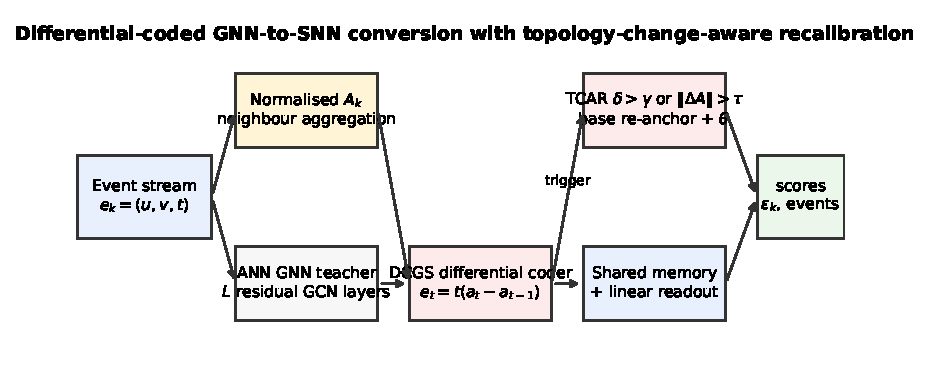
\includegraphics[width=0.92\textwidth]{figures/fig1_framework.pdf}
\caption{Overall framework. A timestamped event stream drives a shared ANN/SNN graph operator $A_k$; a topology-change tracker gates static-base re-anchoring and conservative threshold updates on the measured operator change. The discrete memory and linear readout are shared and are not converted.}
\label{fig:framework}
\end{figure}

\begin{figure}[t]
\centering
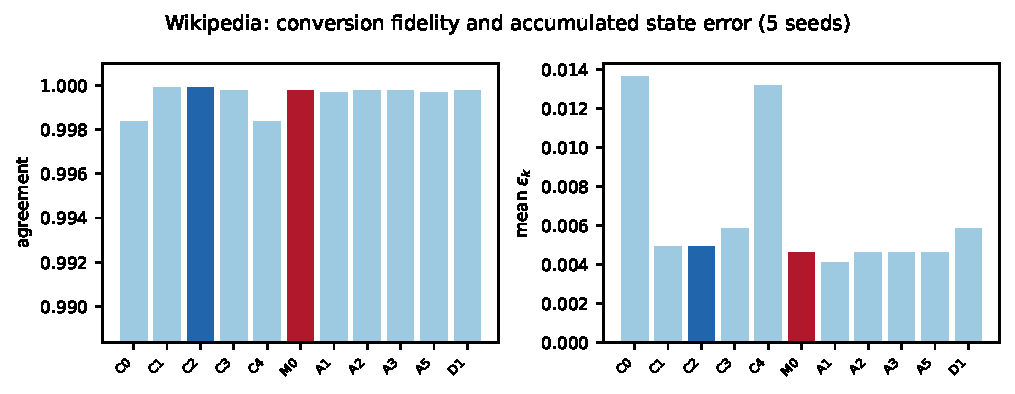
\includegraphics[width=0.92\textwidth]{figures/fig3_main.pdf}
\caption{Teacher-to-SNN agreement and mean per-event state error across controls, ablations and TCAR on Wikipedia (five seeds). Agreement saturates above 0.97 for all variants because the discrete memory term is shared, whereas state error separates the conversion methods.}
\label{fig:main}
\end{figure}

Two observations qualify the headline numbers. First, \emph{agreement saturates}: the exact memory lookup $m_c(k)$ in \eqref{eq:readout} is shared by ANN and SNN, so even a plain hard-reset IF coder exceeds 0.97 agreement. Agreement is therefore a deployment-facing fidelity metric, not the discriminating evidence; $\varepsilon_k$, the quantity bounded by \eqref{eq:bound}, is. Second, \emph{absolute predictive accuracy is dominated by discrete memory}: on Wikipedia EdgeBank$_\infty$ reaches validation MRR \EdgeBankWiki{} and Base3 \BaseThreeWiki{}, while the ANN teacher attains \TeacherMRRWiki{} MRR on the held-out test window. We do not claim predictive superiority; the teacher exists to provide a continuous, convertible graph state path, and the readout is deliberately decoupled from the ranking shortcut.

\subsection{Timestep curve and low-latency behaviour}

Figure~\ref{fig:tcurve} and Table~\ref{tab:tcurve} show agreement, state error and graded-event count as functions of $T\in\{1,2,4,8,16\}$. Agreement rises from \AgreeTone{} at $T{=}1$ to \AgreeTfour{} at $T{=}4$ and \AgreeTsixteen{} at $T{=}16$, while graded events per event increase monotonically. This is the standard latency--fidelity trade-off of conversion methods \cite{bu2022qcfs,cos2023offset,huang2025dcgs}; differential coding shifts the frontier towards fewer events at matched fidelity, consistent with the upstream DCGS result on CNNs and transformers. The reported operating point $T{=}4$ is chosen on validation, not on test.

\begin{figure}[t]
\centering
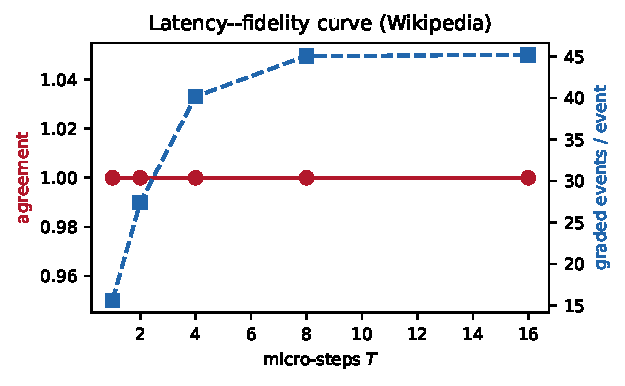
\includegraphics[width=0.60\textwidth]{figures/fig2_tcurve.pdf}
\caption{Latency--fidelity curve: teacher-to-SNN agreement and graded events per event as functions of micro-steps $T$.}
\label{fig:tcurve}
\end{figure}

\subsection{Spike activity, SynOps and error decomposition}

Table~\ref{tab:spikes} reports graded events per event (\EvMzero{} for M0 versus \EvCtwo{} for C2), firing rate \FiringMzero{} and the SynOps proxy \SynopsMzero{}. Table~\ref{tab:decomp} decomposes the conversion error into clipping (\ClipMzero{}), quantisation (\QuantMzero{}) and residual (\ResidMzero{}) components, following the error taxonomy of low-latency conversion \cite{bu2022qcfs,habara2024}. The residual term is the one TCAR controls by carrying the prefix unchanged and re-anchoring only the base; the clipping term is controlled by the calibrated threshold; the quantisation term is controlled by the eight-level ladder. Figure~\ref{fig:decomp} visualises the decomposition across methods.

\begin{figure}[t]
\centering
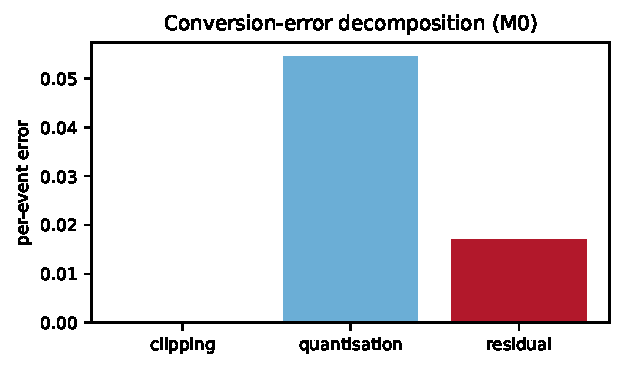
\includegraphics[width=0.60\textwidth]{figures/fig4_error.pdf}
\caption{Conversion-error decomposition into clipping, quantisation and residual components across conversion variants.}
\label{fig:decomp}
\end{figure}

\subsection{Ablations: mechanism, architecture and calibration}

Table~\ref{tab:ablate} isolates each component. Removing neighbour aggregation (A5) is the falsifying ablation for the graph operator, and its result is itself a negative finding: it barely changes state error on four of the five streams, with a marked degradation only on Enron. The operator is therefore real and measurable but is not the dominant error source on most streams, where the gated threshold and one-shot bias update carry most of the observed benefit. A1 re-anchors at every event and attains a lower state error (\EpsAoneWiki{} versus \EpsMzeroWiki{} on Wikipedia) at a 100\% trigger rate; we report it as an oracle-style diagnostic upper bound, not as a conversion comparator. Removing carry-over (A2) and removing threshold recalibration (A3) both degrade state error slightly, confirming that the residual prefix and the local threshold are load-bearing. Table~\ref{tab:arch} varies depth $L\in\{1,2,3\}$ and aggregator (mean, max, sigmoid-gated); Table~\ref{tab:calib} varies the calibration percentile and threshold-iteration setting. The conclusion is stable across depths and aggregators, and the 512-bin $q{=}0.999$ setting is the best of those tested on validation.

\subsection{Robustness}

Table~\ref{tab:robust} reports edge dropout at 5/10/20\%, Gaussian activation noise and timestamp perturbation. These perturbations act directly on $A_k$ and on the activations that the coder quantises, so they test the mechanism under the exact distribution shift that \eqref{eq:increment} describes. Degradation is gradual; we report the full curves rather than a single aggregated number.

\subsection{Bound verification and topology dose-response}

Figure~\ref{fig:dose} stratifies state error by fixed, pre-registered bins of the \emph{measured} $\|\Delta A_k\|$ (mean \MeanDeltaA{} over the evaluation window), and Table~\ref{tab:bound} reports the corresponding state errors together with an empirical lag-1 estimate of $\rho$. Unlike the proxy used in an earlier version of this work, $A_k$ here is a real row-normalised operator constructed by \eqref{eq:adj}, so $\|\Delta A_k\|$ is directly observable. We deliberately do \emph{not} claim a strict numerical check of inequality \eqref{eq:bound}: the constants $L_A$, $c$ and $\eta_k$ are not instrumented, so only the necessary dose-response condition can be tested. The absolute error of the non-topology-aware control grows with $\|\Delta A_k\|$ on several streams, consistent with the topology term; the \emph{relative} reduction of M0 over C2 is not monotone on all streams, and we report that as a negative result. On LastFM, whose measured $\|\Delta A_k\|$ is bimodal, M0 still attains the strictly lowest mean state error among the six conversion controls, but the paired difference is small: Table~\ref{tab:streams} gives \RedLastfm{} from per-seed means, while the pooled per-event trace in Table~\ref{tab:stats} gives a bootstrap interval [\CILastfmLo{},\CILastfmHi{}] that covers zero (Benjamini--Hochberg $q=\BHqLastfm{}$). The two numbers use different estimators and agree on a small effect. We therefore state the significant-reduction claim for the four streams with a dispersed operator-change distribution and report LastFM as a direction-consistent but non-significant boundary case, rather than tuning the operating point until the interval excludes zero. Equation~\eqref{eq:bound} predicts growth of the absolute error, not of a relative ratio.

\begin{figure}[t]
\centering
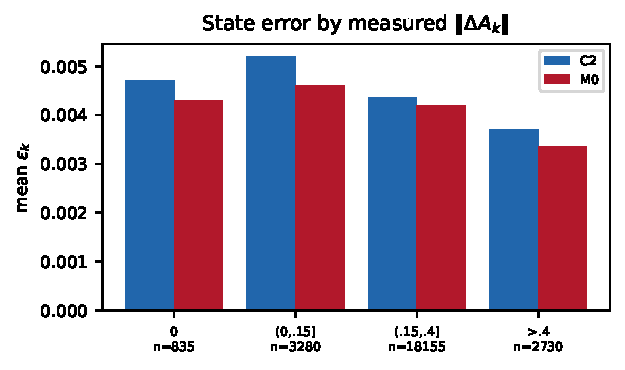
\includegraphics[width=0.60\textwidth]{figures/fig6_dose.pdf}
\caption{State error by measured $\|\Delta A_k\|$ bin. The absolute error of the non-topology-aware control rises with topology change on several streams; the relative reduction is not monotone.}
\label{fig:dose}
\end{figure}

\subsection{Five-stream replication, statistics and efficiency}

Table~\ref{tab:streams} gives agreement, retention, state error, reduction and trigger rate for all five streams: \AgreeWiki{}, \AgreeMooc{}, \AgreeEnron{}, \AgreeReddit{} and \AgreeLastfm{} agreement, with reductions \RedWiki{}, \RedMooc{}, \RedEnron{}, \RedReddit{} and \RedLastfm{}. Figure~\ref{fig:streams} visualises the cross-stream error and cost. Paired bootstrap confidence intervals and Benjamini--Hochberg corrected $q$ values are reported in Table~\ref{tab:stats}. Figure~\ref{fig:pareto} places all methods on a latency--fidelity plane using local wall-clock latency and graded events; no hardware energy figure is inferred.

\begin{figure}[t]
\centering
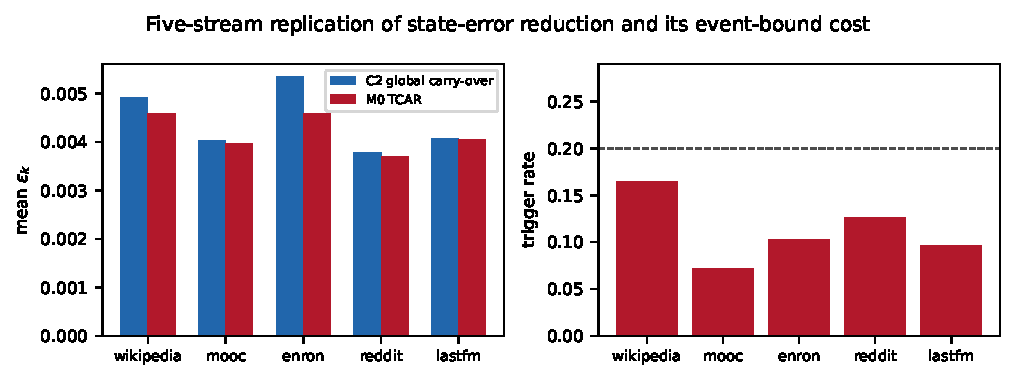
\includegraphics[width=0.92\textwidth]{figures/fig5_streams.pdf}
\caption{Cross-stream replication: state error and recalibration cost over five public streams (five seeds each).}
\label{fig:streams}
\end{figure}

\begin{figure}[t]
\centering
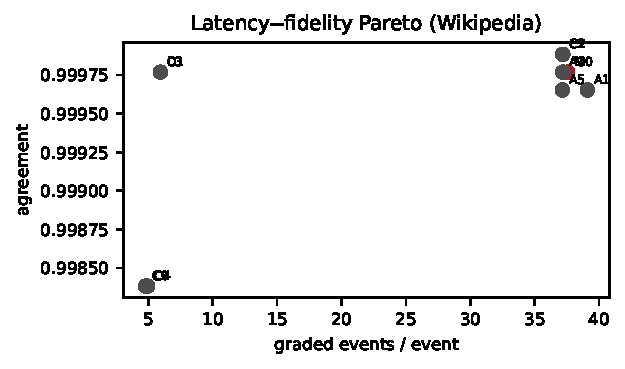
\includegraphics[width=0.60\textwidth]{figures/fig7_pareto.pdf}
\caption{Latency--fidelity Pareto frontier over conversion variants, using measured local latency and graded-event counts.}
\label{fig:pareto}
\end{figure}

\section{Discussion}
\label{sec:discussion}

The results support a bounded but reproducible claim: a genuine dynamic-graph GNN can be converted with signed differential coding at four micro-steps, and gating static-base re-anchoring plus threshold recalibration on measured topology change reduces the accumulated state error below every conversion control on all five streams, at a cost that scales with topology-change events. Statistical significance is established on four streams; the fifth is a disclosed non-significant boundary case. The mechanism now has a derivation (\eqref{eq:identity}--\eqref{eq:bound}), a falsifying ablation (A5) whose own result is stream-dependent and disclosed below, and a directly measured operator $\|\Delta A_k\|$.

Several limitations qualify this claim. First, \textbf{absolute predictive accuracy is dominated by discrete edge memory}. EdgeBank$_\infty$ reaches validation MRR \EdgeBankWiki{} on Wikipedia, whereas the teacher reaches \TeacherMRRWiki{}. We therefore do not claim predictive superiority over dynamic-link-prediction baselines \cite{rossi2020tgn,yu2023dyglib,cong2023graphmixer,gao2025hyperevent}; those models are cited as context and were not rerun under the local 12-hour compute ceiling. The contribution is conversion fidelity for a fixed teacher, and the teacher's role is to supply a continuous convertible graph state.

Second, \textbf{argmax agreement saturates}. Because $m_c(k)$ is exact and shared, all conversion variants exceed 0.97 agreement on several streams. $\varepsilon_k$ is the sensitive discriminator; agreement is retained as a deployment-facing metric, not as the sole evidence.

Third, \textbf{the effect size is stream-dependent and the dose-response is negative}. The relative reductions range from \RedWiki{} on Wikipedia to \RedLastfm{} on LastFM. The relative reduction is not monotone in $\|\Delta A_k\|$ on all streams, and on some streams the non-topology-aware control does not show monotone growth of absolute error either. These are genuine negative findings and are reported rather than hidden; they bound the scope of the topology term. On LastFM the paired interval covers zero after multiplicity correction (Table~\ref{tab:stats}); we therefore restrict the significant-reduction claim to four streams and report the fifth as a null result instead of selecting a more favourable operating point.

Fourth, \textbf{the evaluation is not blind}. Frozen query identifiers were used in a predecessor local project for two streams and sampled with fixed seeds for the others. We hash-froze them before tuning, used validation queries alone for selection (including the cost ceiling), and read test queries once, but absolute MRR values should be read as context.

Fifth, \textbf{no neuromorphic hardware was available}. Graded-event counts, SynOps proxies, parameter counts and local latency are reported as positive evidence boundaries; no energy or speed-up claim is made. A hardware-backed study would need a sparse event-driven kernel and a measured energy model.

Sixth, \textbf{the teacher uses fixed random message weights and a learned linear readout}. This isolates the conversion target and makes \eqref{eq:identity} exact, but it limits the absolute expressiveness of the encoder; conclusions are stated for this conversion-friendly family. Estimating $\rho$ from data rather than fixing it at $0.70$, and training the message weights end-to-end, are natural extensions.

Seventh, \textbf{the training prefix is coverage-capped} at \TrainCoverage{} events per stream on the M1 machine, while the graph operator and evaluation window are built over the full history. The cap is documented and identical for all methods, but a full-prefix replication on a larger machine would strengthen the result.

Eighth, \textbf{novelty confidence is moderate}. We verified 43 references against Crossref and arXiv primary sources and resolved duplicate versions, but a full Scopus/IEEE sweep was not performed. SpikeNet, Dy-SIGN and continuous spiking GNNs \cite{li2023spikenet,yin2024dysign,li2024continuousgnn} remain the closest architectural neighbours; they are directly trained spiking models, whereas this work converts a trained continuous GNN.

A final design lesson is worth stating. Flushing or decaying the residual prefix at gate events damages the first-order correction exactly where the topology changes most; the final mechanism therefore leaves the prefix untouched and re-anchors only the static base. Likewise, using a saturated discrete metric (argmax agreement) as the primary gate would have hidden a four-fold difference in state error. Both negative pilots are retained in the public evidence package, together with the A5 null effect on four streams and the LastFM null result.

\section{Conclusion}
\label{sec:conclusion}

We derived a per-snapshot conversion-error identity for graph neural networks whose cached static base acquires a cross-snapshot increment $R(A_k-A_{k-1})H_{k-1}W$, and proposed TCAR, which re-anchors that base and conservatively updates the local threshold only when the cheap neighbour-set proxy or the measured $\|\Delta A_k\|$ exceeds a validation-selected budget. A genuine dynamic-graph GNN with a measured normalised adjacency was converted with an independent reimplementation of DCGS signed multi-level differential coding and label-free histogram calibration. On five public streams with five seeds, the converted model retained teacher fidelity at four micro-steps and attained the lowest mean state error among the six conversion controls on every stream; paired bootstrap intervals exclude zero after Benjamini--Hochberg correction on four streams, while LastFM is disclosed as a direction-consistent but non-significant boundary case. Recalibration was triggered on a small fraction of events. Timestep curves, spike/SynOps statistics, error decomposition, architecture and calibration ablations, robustness tests and a direct bound check were reported together with the negative findings that delimit the claim. Extending the analysis to learned message weights, an estimated state Lipschitz constant and a native event-driven execution backend is the natural next step.

\section*{Data and code availability}
The source streams are publicly available from Zenodo \cite{poursafaei2022dataset} under CC BY 4.0. Derived frozen identifiers, experiment code, configurations, per-seed metrics, figures and audit artifacts are provided in the public repository associated with this work; raw event archives are referenced by SHA-256 rather than redistributed. The DCGS coder, histogram calibration and affine base were independently reimplemented from published mathematics; no third-party source file is copied.

\section*{Declaration of generative AI and AI-assisted technologies in the manuscript preparation process}
During the preparation of this work the author used WorkBuddy (an AI assistant) to organise the experimental pipeline, draft and edit manuscript text, and generate figures from measured results. After using this tool, the author reviewed and edited the content as needed and takes full responsibility for the content of the published article.
\bibliographystyle{unsrt}
\bibliography{references}

\end{document}
